\hypersetup{pdfborder=0 0 0}


\newpage

%%%%%%%%%%%%%%%%%%%%%%%%%%%%%%%%%%%%%%%%%%%%%%%%%%%%%%%%%%%%%%%%%%%%%%%%%%%
\section{Numerical Test Cases}

\subsection{Algorithm and determination of global diffusion coefficient}
Following Winters 1995, first is determined available volume at each depth V(z), then for each time-step build the reference profile by filling V(z) from the bottom up starting with the densest parcels.

Background Potential Energy and its evolution is computed from resulting z*(rho). This is compared to the computed terms of right-hand side of eq (...) to estimate the diffusive coefficient, in the algorithm assumed to be spatially homogeneous and isotropic $\kappa_h=\kappa_v=\kappa$ (can be considered accurate in realistic oceanic cases as long as resolution of gradients is the same) but can evolve through time.



\begin{subequations}
  \begin{alignat}{2}
  \displaystyle 
 	&\frac{d E_b}{d t} &&= \quad g\int_x \int_{-1}^0 \rho h \frac{\partial z^*}{\partial t}\bigg\rvert_{xs} \ dx ds\\
 	& &&\quad +g\int_x \int_{-1}^0\rho v_s \frac{\partial z^*}{\partial s}\bigg\rvert_{tx} \ dx ds
+g\int_x \int_{-1}^0 \rho h u \frac{\partial z^*}{\partial x}\bigg\rvert_{ts} \ dx ds \\
 & && \quad - g\bigg[ \int_{-1}^0 \rho h z^* u \ ds\bigg]_{x} - g\bigg[ \int_x\rho z^* v_s \ dx\bigg]_0^1 \\
 & && \quad + g\bigg[ \int_{-1}^0 h z^* \kappa^h \frac{\partial \rho}{\partial x}\bigg\rvert_{ts} \ ds \bigg]_{x}
 - g\int_x \int_{-1}^0 h \kappa^h \frac{d z^*}{d \rho} \frac{\partial \rho}{\partial x}\bigg\rvert_{ts}^2 \ dx ds \\
 & && \quad + g\bigg[ \int_x z^* \frac{\kappa^v}{h} \frac{\partial \rho}{\partial s}\bigg\rvert_{tx} \ dx \bigg]_0^1
 - g\int_x \int_{-1}^0 \frac{\kappa^v}{h} \frac{d z^*}{d \rho} \frac{\partial \rho}{\partial s}\bigg\rvert_{tx}^2 \ dx ds
\end{alignat}
\end{subequations}


\begin{subequations}
  \begin{alignat}{2}
  \displaystyle 
 	&\frac{d E_b}{d t} &&= \quad \underbrace{g\int_x \int_{-1}^0 \rho h \frac{d z^*}{d t}\bigg\rvert_{xs} \ dx ds}_{?\phi_S? ou F_S?}\\
 %	& &&\quad +g\int_x \int_{-1}^0\rho v_s \frac{\partial z^*}{\partial s}\bigg\rvert_{tx} \ dx ds
%+g\int_x \int_{-1}^0 \rho h u \frac{\partial z^*}{\partial x}\bigg\rvert_{ts} \ dx ds \\
 & && \quad \underbrace{- g\bigg[ \int_{-1}^0 \rho h z^* u \ ds\bigg]_{x} - g\bigg[ \int_x\rho z^* v_s \ dx\bigg]_0^1}_{F_A} \\
 & && \quad \underbrace{+ g  \kappa \ \bigg[ \int_{-1}^0 h z^*  \frac{\partial \rho}{\partial x}\bigg\rvert_{ts} \ ds \bigg]_{x}
 + g \kappa \ \bigg[ \int_x z^* \frac{1}{h} \frac{\partial \rho}{\partial s}\bigg\rvert_{tx} \ dx \bigg]_0^1 }_{\kappa F_D}\\
 & && \quad \underbrace{- g \kappa \int_x \int_{-1}^0 h  \frac{d z^*}{d \rho} \frac{\partial \rho}{\partial x}\bigg\rvert_{ts}^2 \ dx ds 
 - g \kappa \int_x \int_{-1}^0 \frac{1}{h} \frac{d z^*}{d \rho} \frac{\partial \rho}{\partial s}\bigg\rvert_{tx}^2 \ dx ds}_{\kappa \phi_D}
\end{alignat}
\label{bilanBPEal}
\end{subequations}

Note $D=F_D+\phi_D$

Therefore with eq \ref{bilanBPEal}a and b  as non-diffusive terms and c and d as diffusive terms :
\begin{equation}
\kappa = \frac{\frac{dE_b}{dt} \ - \ \text{non-diffusive terms}}{\text{diffusive terms}}=\frac{\frac{dE_b}{dt}-(\phi_S+F_A)}{D}
\end{equation}

Another way is to search recursively for the best coefficient $\kappa$ that will minimize error over time-interval 2n

$ \sum\limits_{i_0-n}^{i_0+n} (\frac{dE_b^i}{dt}-(\text{non-diffusive terms}^i + \kappa^{i_0} * \text{diffusive terms}^i))^2$


\subsection{NUMLAB experiment}
2D Simple advection-diffusion code, cyclic in each direction. RK3-UP3 with harmonic diffusion unless stated otherwise. 

Evolution of BPE and right-hand terms are computed as FW-C2...

No change in volume so right-hand term of eq. \ref{bilanBPEal}.a integrate to zero for all Numlab cases. No vertical velocity, $v_s=0$, so first term of \ref{bilanBPEal}.b and second term of \ref{bilanBPEal}.c are zero.

Initial tracer field is either $\psi(x)=cos(2\pi x/L_x)$ or $\psi(x,z)=Re(e^{i2\pi x/L_x}e^{i 2 \pi z/L_z})$. Parameters are $dx=0.5$ m, $dz=0.5$ m, $L_x=30$ m, $L_z=20$ m, $dt=0.1s$ and table.


\begin{table}[h!]
\centering
\begin{tabular}{|l|l|l|l|}
\hline
Name & $\psi_0$ & $\kappa$ (m$^2$/s)& U(m/s)\\
\hline
diffVH & $\psi(x,y)$ & 10$^{-3}$& 0\\
diffVHx & $\psi(x,y)$ & $\kappa$(x) & 0\\
IMP & $\psi(x,y)$ & Impl & 0.1\\
ADV & $\psi(x)$ & Impl & $4.10^{-5}$\\
\hline
\end{tabular}
\caption{Parameters of simulation}
\end{table}

\subsubsection{Homogeneous diffusion case : diffVH}
Basic reference test case without horizontal velocity

possibility of flux through the horizontal boundary so first term of \ref{bilanBPEal}.e can be be non-zero.

\begin{figure}[h!]
\centering
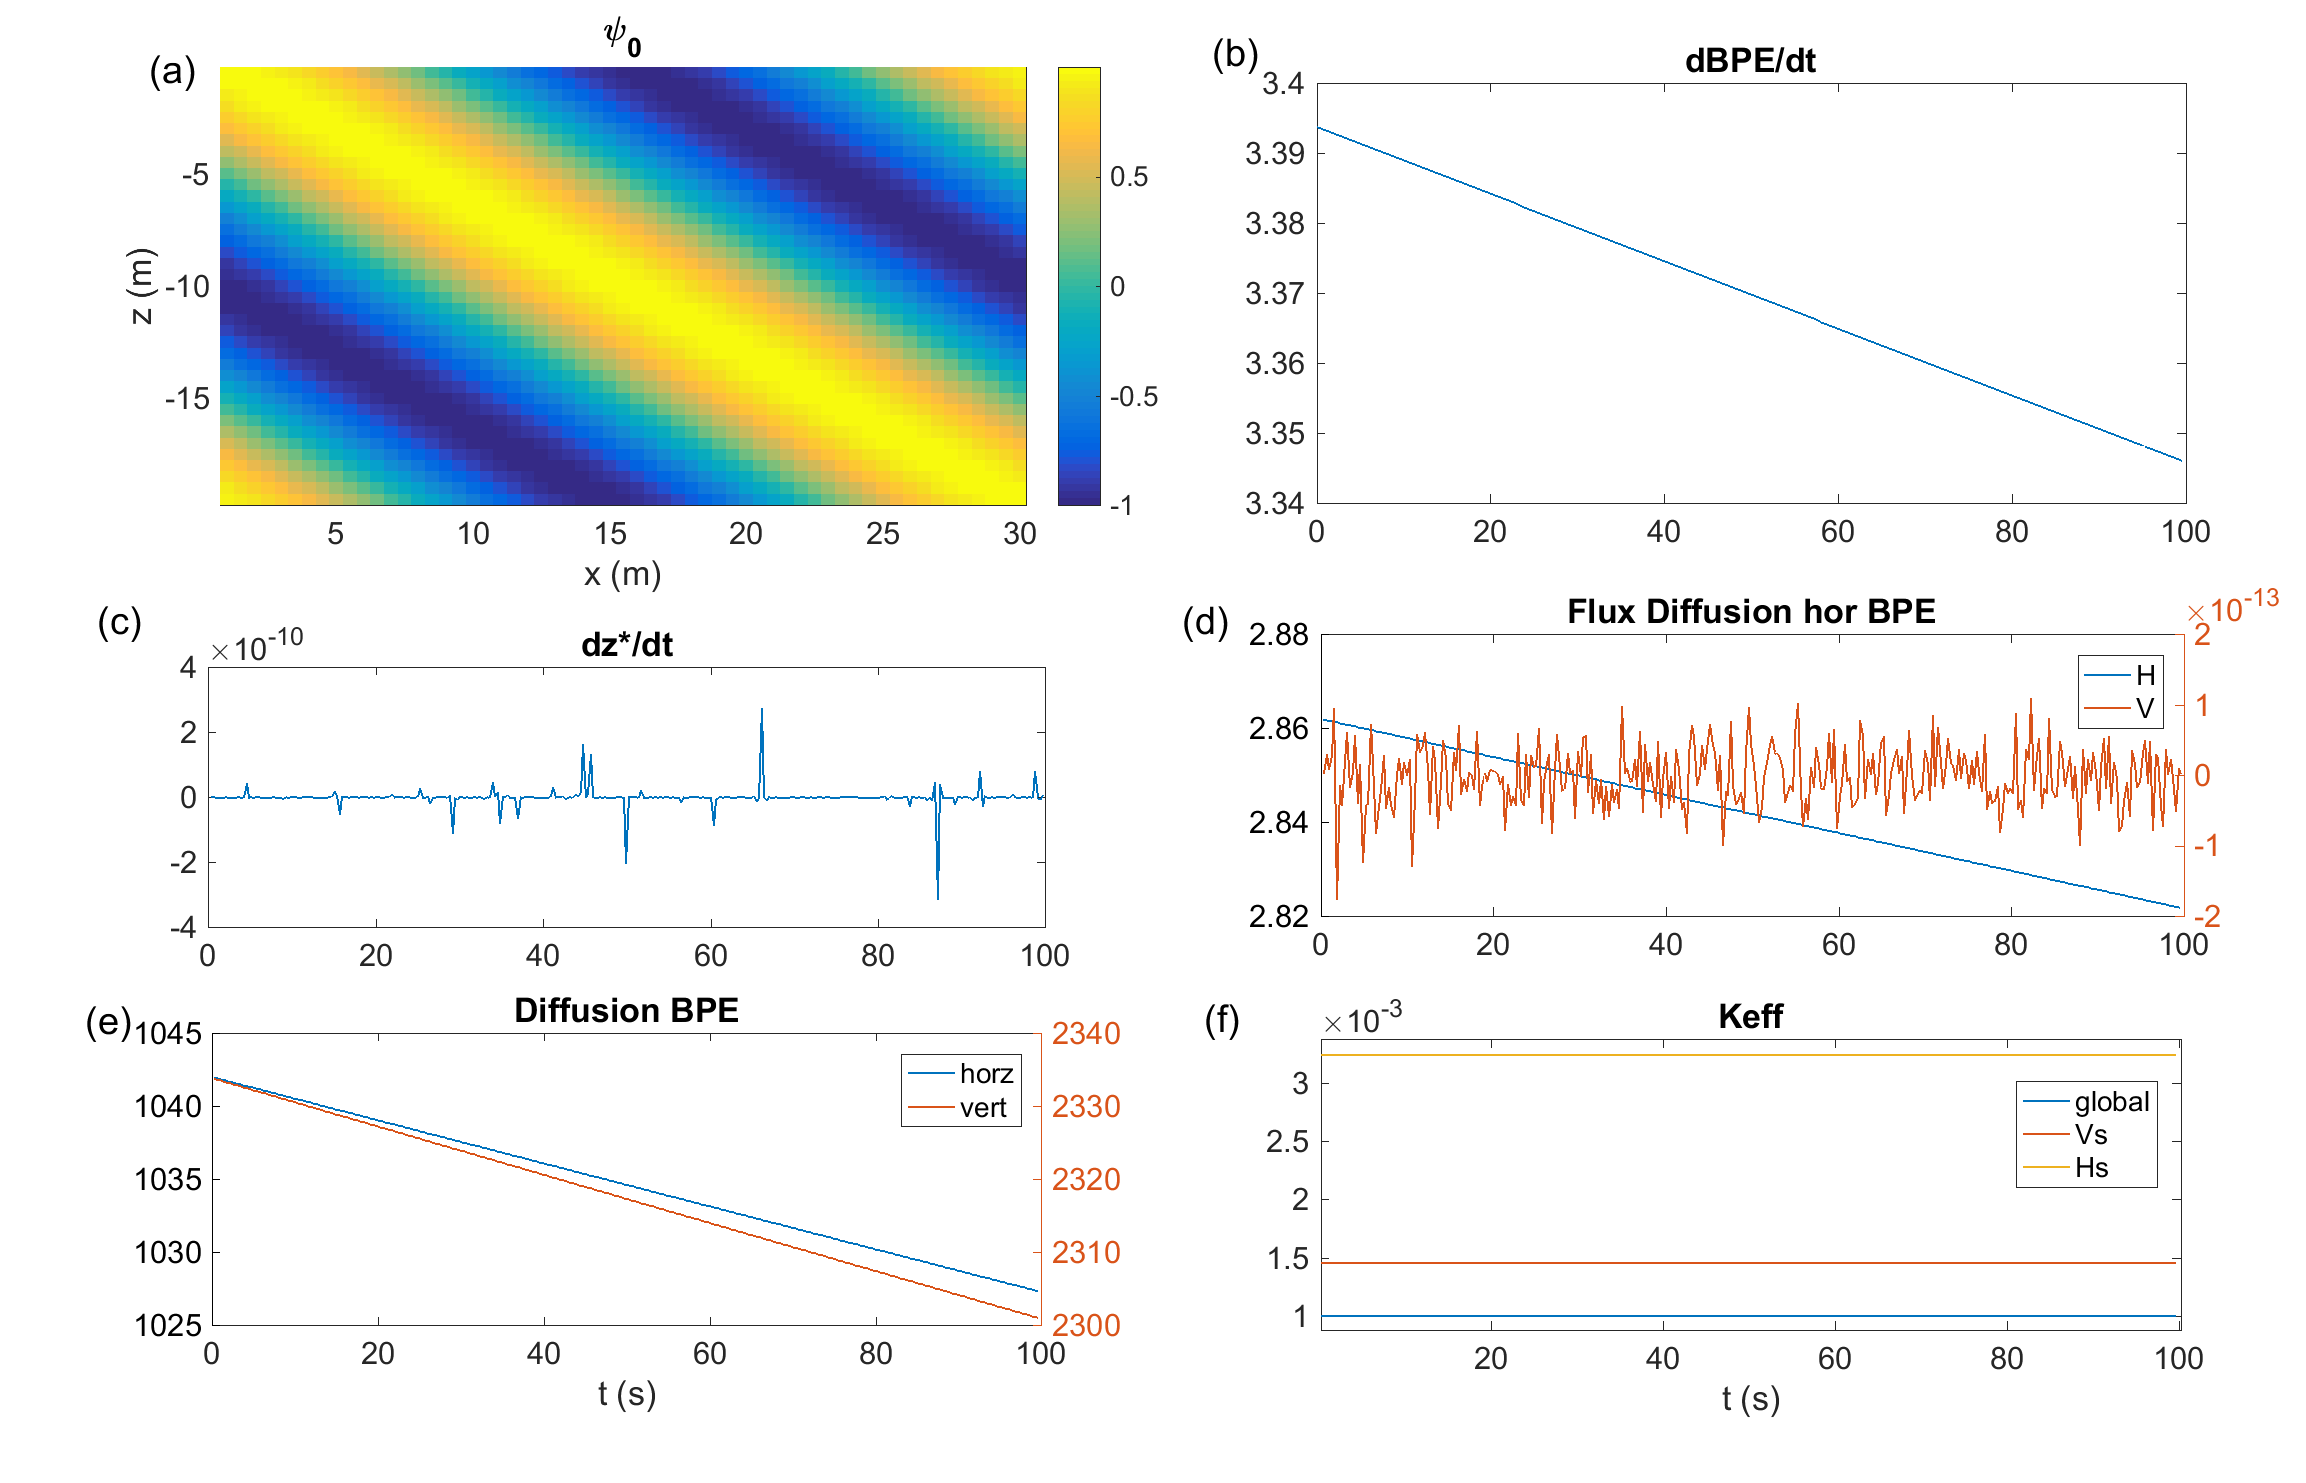
\includegraphics[width=1\textwidth]{./CHAP_BPE/AGBPE_numlab1.png}
\caption{blablabla}
\label{fig1numlab}
\end{figure}

Figure \ref{fig1numlab} (c) is sum of right-hand terms of eq. \ref{bilanBPEal}a and \ref{bilanBPEal}b. (d) and (e) are diffusive terms respectively terms \ref{bilanBPEal}d and \ref{bilanBPEal}e separated in vertical and horizontal gradient contribution, without factoring $\kappa$.

Figure \ref{fig1numlab} (f) is value of diffusion coefficient, in blue for $\kappa_v=\kappa_h=\kappa$ and find expected value, red if $\kappa_h=0$ in equation, yellow if $\kappa_v=0$, ie. the observed diffusion can also be explained by purely horizontal or vertical diffusion but coefficient would be stronger.

\subsubsection{Local diffusion case : diffVHx}

\begin{figure}[h!]
\centering
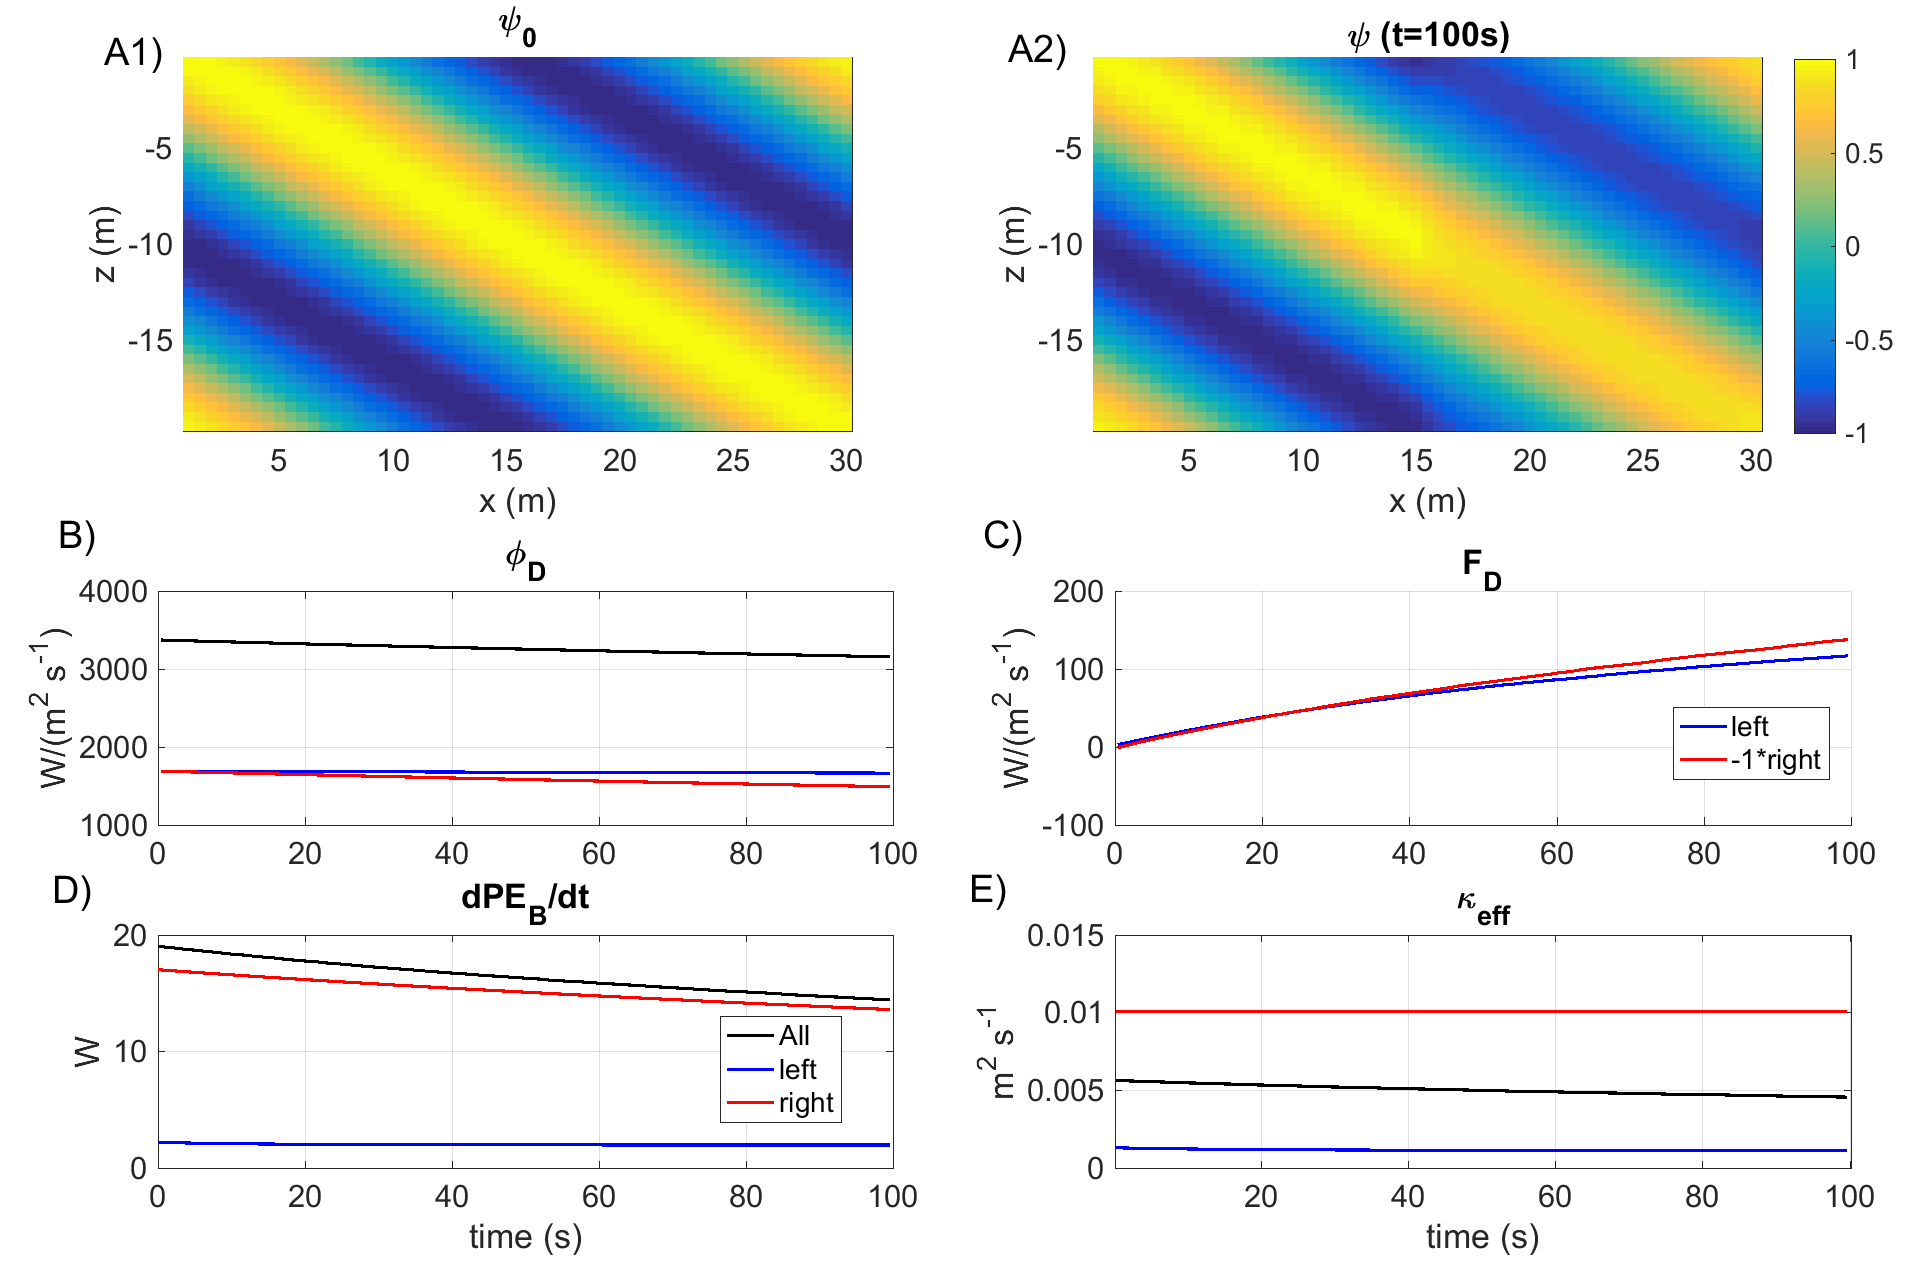
\includegraphics[width=1\textwidth]{./CHAP_BPE/AGBPE_numlab2.png}
\caption{(c) is \ref{bilanBPEal}e}
\label{fig2numlab}
\end{figure}

Initial tracer field same as in fig \ref{fig1numlab}.

For x$<$15 m, $\kappa = 10^{-3}$, otherwise $\kappa = 10^{-2}$ m$^2$/s.

Diffusion coefficient has different value along the horizontal axis, effect of using algorithm on each half-domain or entire domain. The value z*(rho) of a given density is dependant on the breadth of the domain where the reference profile is constructed. (only takes into account the densities in this domain). So the right-hand sides term of the BPE evolution equation will change. Particularly this enables to take into account spatial variabiity of $\kappa$.

Coefficient computed over all the domain is an average.

The diffusion terms do not cancel each other since z* is different on each half.

\subsubsection{Implicit diffusion case : IMP}

With $\psi(x,t=0)=cos(2\pi x/L_x)$, solution of advection-diffusion problem is : $\psi(x,t)=e^{-\kappa k_x^2 t}cos(k(x-Ut))$ with $k_x=2\pi/L_x$


\underline{\textit{2nd order scheme : UP1}}
\begin{figure}[h!]
\centering
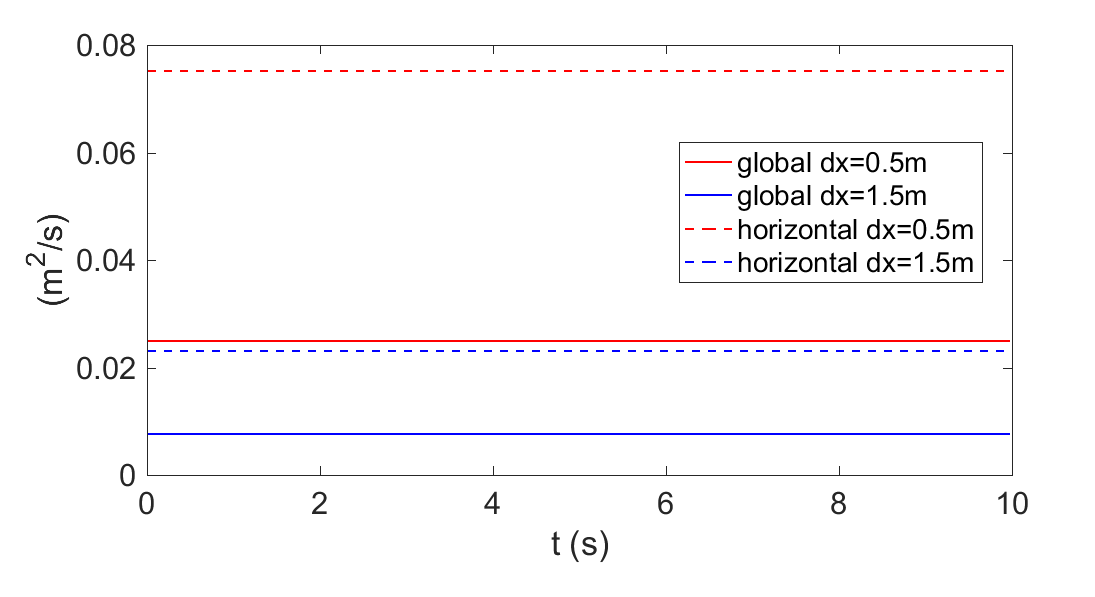
\includegraphics[width=0.5\textwidth]{./CHAP_BPE/AGBPE_numlab3.png}
\caption{Diffusion coefficient for implicit diffusion case}
\label{fig3numlab}
\end{figure}

RK3-UP1 scheme with horizontal velocity. No explicit harmonic diffusion. Development of discrete advection equation gives formulation of an implicit diffusion coefficient $\kappa_{h,i}=\frac{1}{2}U \Delta x$ (ref?)
\begin{equation}
U \frac{\partial \psi}{\partial x} +\frac{\partial \psi}{\partial t} = \frac{1}{2} U \Delta x  \frac{\partial^2 \psi}{\partial x^2} + o(\frac{\partial^3 \psi}{\partial x^3})
\end{equation}
$dx=0.5$ m then $dx=1.5$ m, gives values of $\kappa_{h,i}$ of 0.025m$^2$/s and 0.075m$^2$/s

Find the good value if don't take into account term of vertical diffusion, only along current.\\

\underline{\textit{4th order scheme : UP3}}

RK3-UP3 advection scheme with horizontal velocity. Expending the discrete scheme give 4th order diffusion.
\begin{equation}
U \frac{\partial \psi}{\partial x} +\frac{\partial \psi}{\partial t} = \underbrace{\frac{1}{120}(5 C^3-10) U \Delta x^3}_{k_4}  \frac{\partial^4 \psi}{\partial x^4} + o(\frac{\partial^5 \psi}{\partial x^5})
\end{equation}
where C is the advection Courant number, here $C=2 . 10^{-2}$. Fourth order coefficient is $k_4=-1.10^{-3} m^4/s$. However, the BPE analysis give an implicit diffusion in form of second order with coefficient $k_2=\kappa_{eff}$.

$\kappa_{eff} = \kappa_{exp} + \kappa_{imp}$ is approximated from BPE analysis by minimization of error over the 2 advection cycle duration of simulation (see fig, instantaneous balance give for each case time dependant coefficient, oscillation with amplitude $\approx 4.10^{-5}$ that average to the same $\kappa_{eff}$ value as minimal error proxy). Always find an implicit diffusion of $\approx 4.65.10^{-5} m^2/s$ and by putting the opposite value as explicit diffusion, the effective diffusion is computed as null and can also see that the maximum (or minimum) value of tracer neither increase nor decrease contrary to case with non-zero effective diffusion.


\begin{table}[h!]
\centering
\begin{tabular}{|l|l|l|l|l|l|l|l|l|l|l|}
\hline
$\kappa_{exp}$ & $-10^{-4}$ &$-4.65.10^{-5}$ & $-10^{-5}$& $0$& $10^{-5}$& $10^{-4}$\\
\hline
$\kappa_{eff}$ & $-5.35.10^{-5}$ &$3.5.10^{-8}$ & $3.65.10^{-5}$& $4.65.10^{-5}$& $5.65.10^{-5}$& $14.65.10^{-5}$\\
\hline
$\kappa_{imp}$&\multicolumn{6}{c|}{$4.65.10^{-5}$}\\
\hline
\end{tabular}
\caption{Explicit coefficient given to simulation, effective coefficient computed from BPE analysis and implicit coefficient by deducting one from the other}
\end{table}

\begin{figure}[h!]
\centering
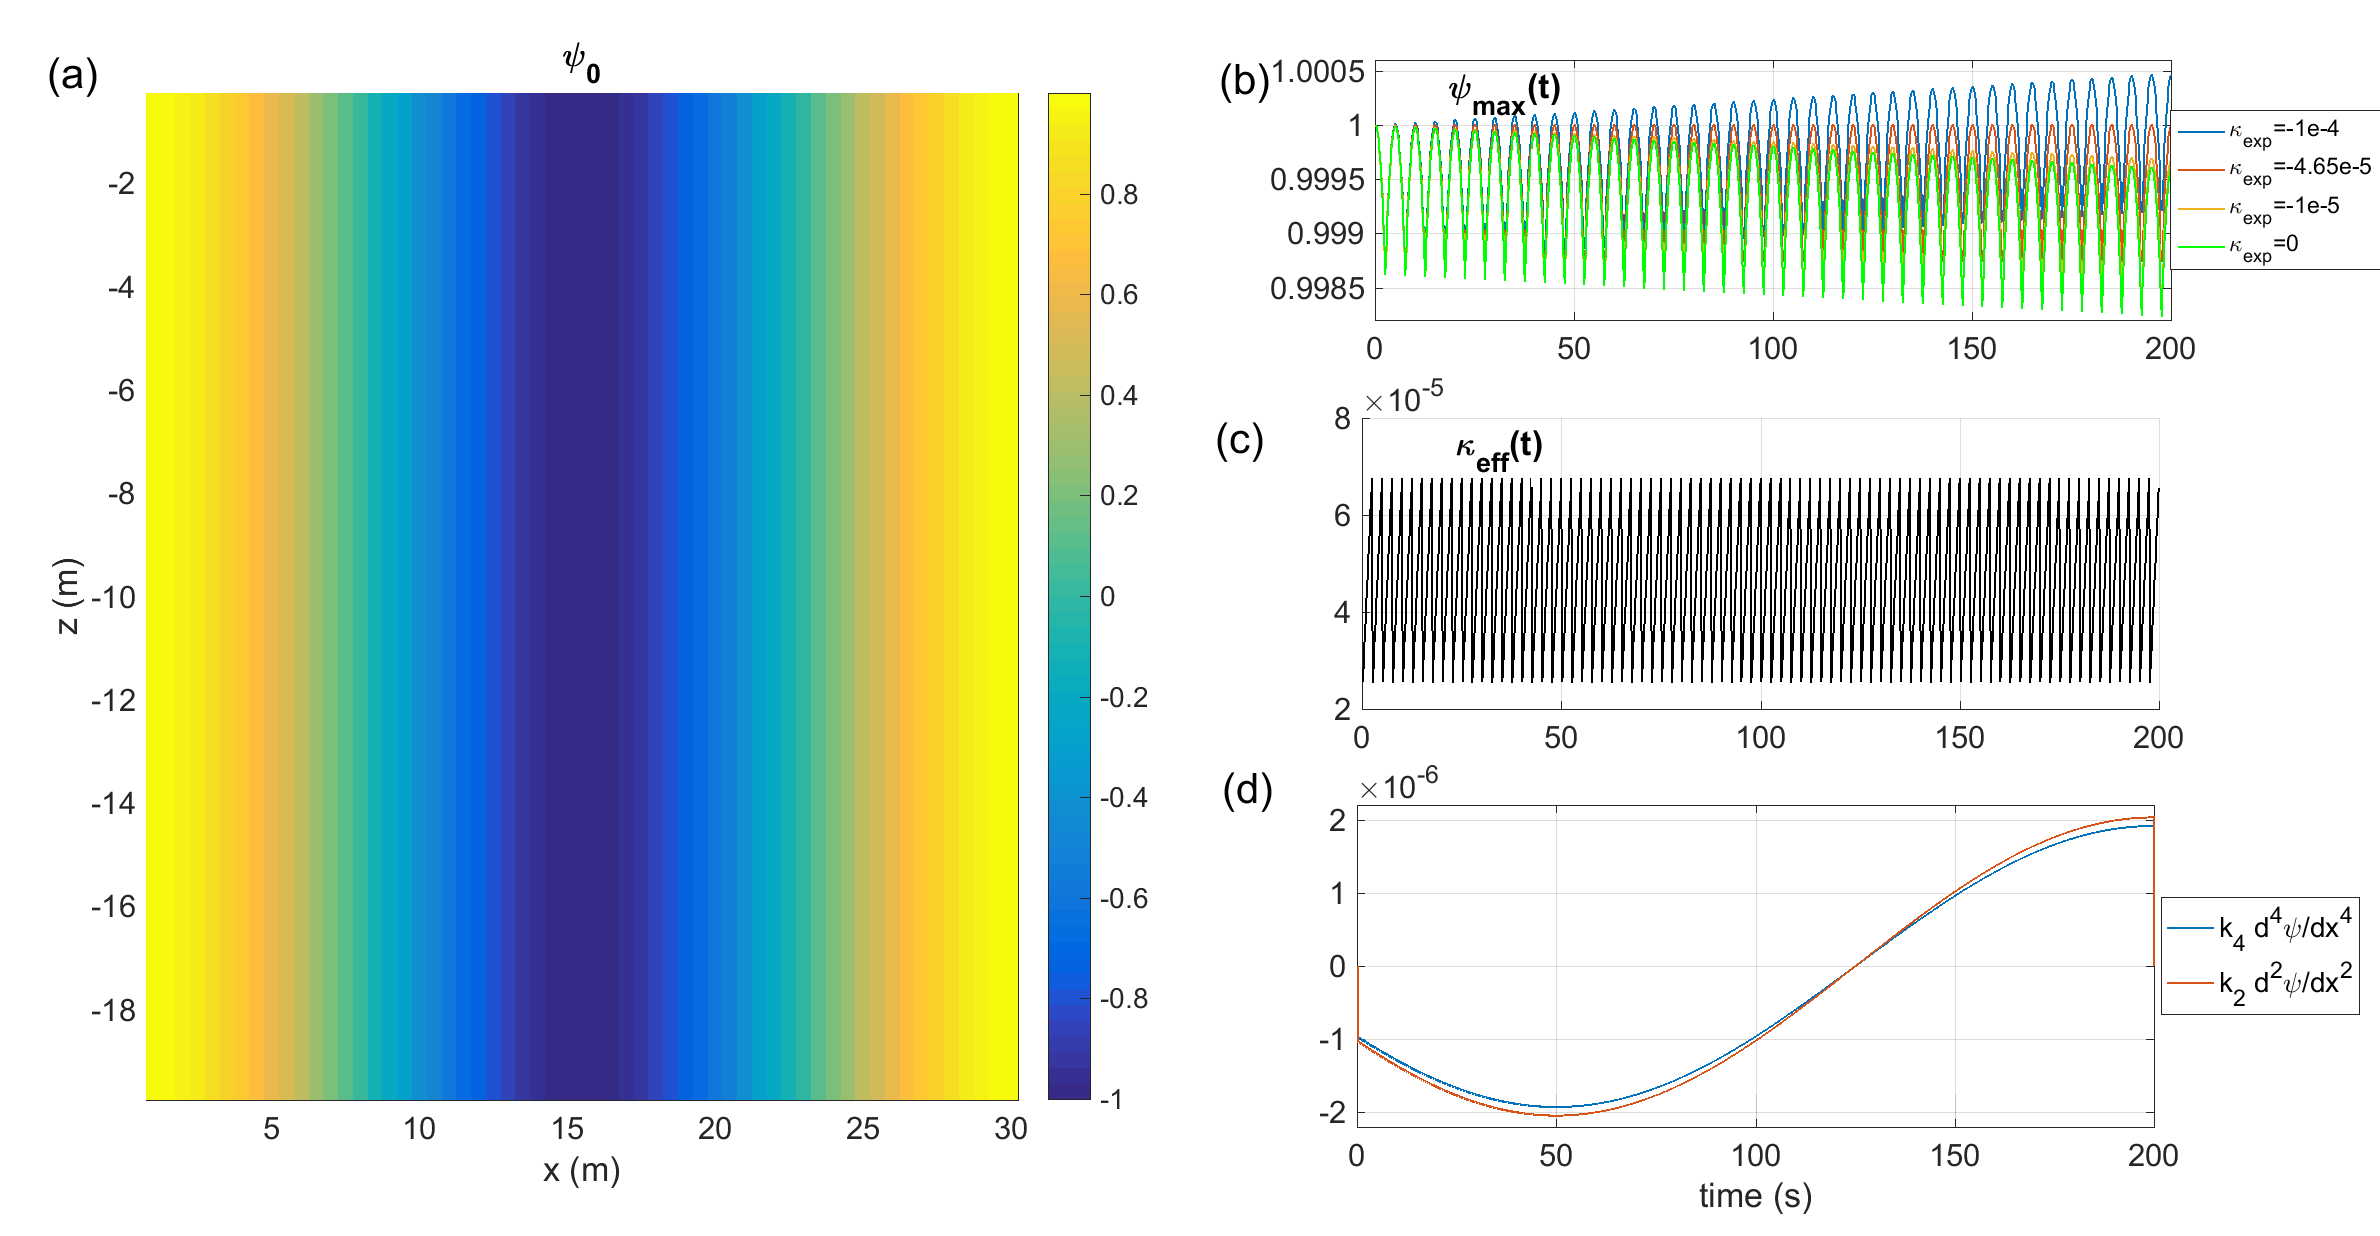
\includegraphics[width=1\textwidth]{./CHAP_BPE/AGBPE_numlab5.png}
\caption{(a) initial field  (b) maximum value of $\psi$ in the field  (c) value of $\kappa{eff}$ by instantaneous balance for case with no explicit diffusion $\kappa{exp}=0$ (d) comparison fourth order and second order formulation}
\label{fig5numlab}
\end{figure}

Take case where $\kappa_{exp}=0$ and compare $k_4 \frac{\partial^4 \psi}{\partial x^4}$ at random point in the domain with second order diffusion with coefficient $2.2 . 10^{-4} m^2/s$ (facteur 5...)

\subsubsection{Local advection and diffusion case : ADV}

\begin{figure}[h!]
\centering
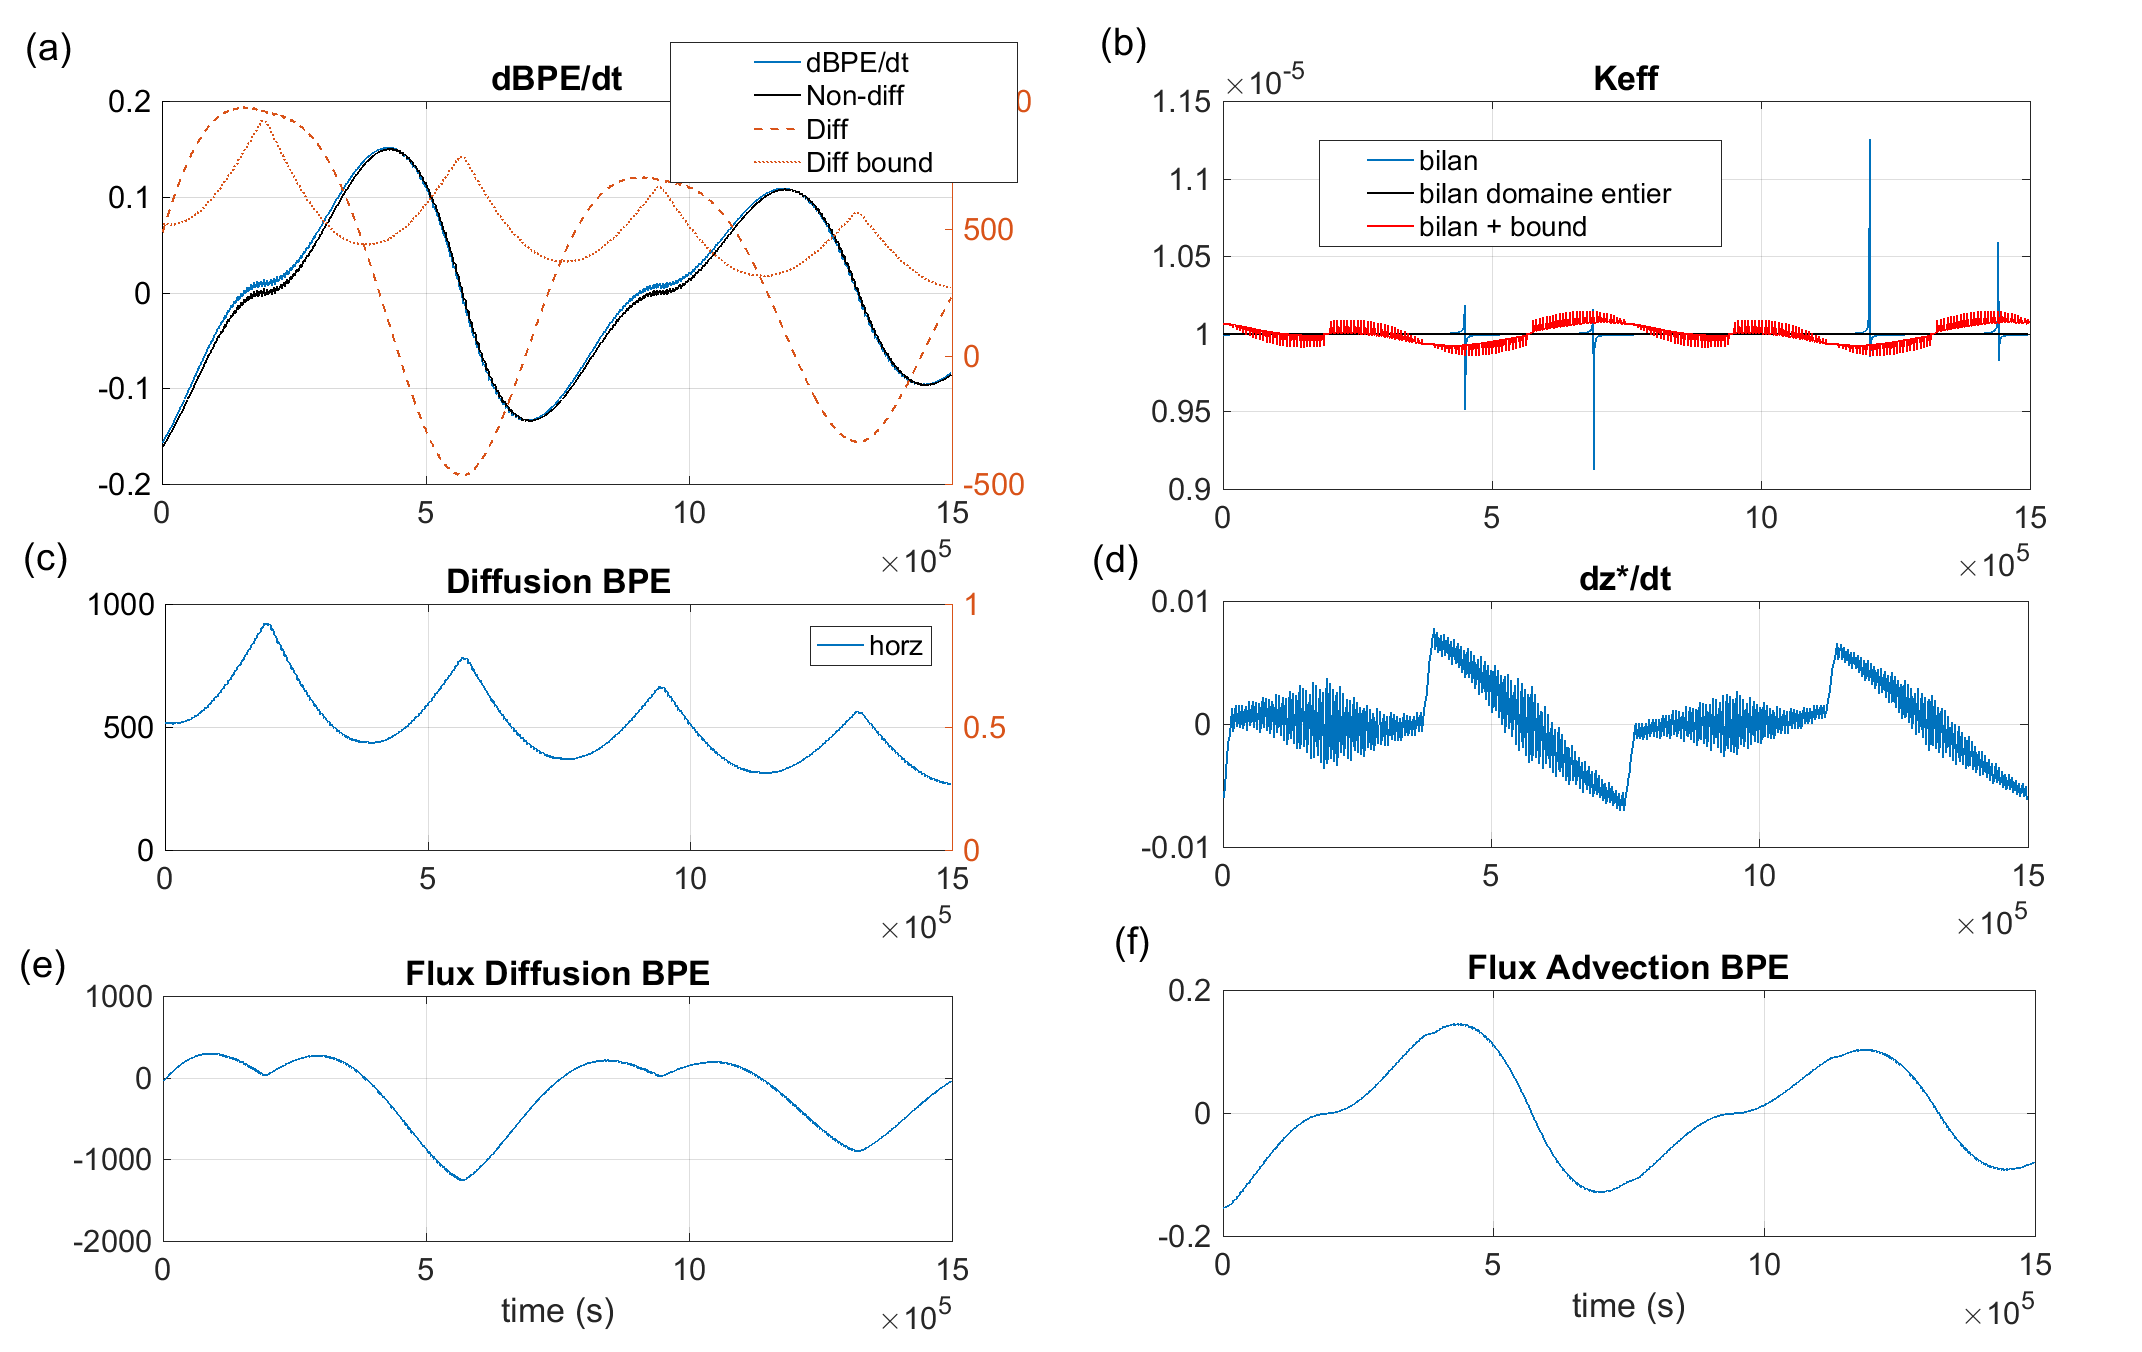
\includegraphics[width=1\textwidth]{./CHAP_BPE/AGBPE_numlab4.png}
\caption{}
\label{fig4numlab}
\end{figure}

Tracer field is $\psi(x)$ as in previous subsection, no vertical gradients contribution. RK3-UP1, no explicit diffusion, only implicit, parameters : dx $=$ 0.5 m, $u=4.10^{-5} m/s$ (dt $=$ 250s) so $\kappa_{imp} = 10^{-5} m^2/s$.


 Look at determination of $\kappa_{eff}$ in left half-domain when both diffusion and advection contribution.
 
 Now have boundary fluxes for both advection (majoritary contribution to right-hand side term in balance) and diffusion. Particularly diffusion fluxes can be negative as entering tracer can act as a source of 'restratification' for the tracer in the volume. Here diffusion in the volume and at the boundary have same size which leads to total diffusion term to sometime be equal to zero and divergence of the balance equation (and so of the value of $\kappa_{eff}$). 
 
 Diffusion term inside the volume however is always strictly positive, can separate the contribution by chosing two different diffusion coefficients for the boundary ($\kappa_{eff}^{bound}$) and the volume ($\kappa_{eff}^{V}$). In figure ... .b $\kappa_{eff}^{bound}$ is taken as the result of the determination of $\kappa_{eff}$ (ie. value for both terms) through the minimization of error method with time interval of 1 advection period (this value is close to the result of the balance equation for the whole domain). Then $\kappa_{eff}^{V}$ is determined by the balance equation with the boundary term put with the non-diffusive terms. This give a non-divergent solution that oscillate around the expected value. (aussi oscillation eval domaine entier mais moins amplitude....)
 
 

%Termes non-diffusifs prépondérants dans le bilan, décalage dû termes diffusifs, pour calcul sur domaine entier retrouve bien $\kappa=10^{-2}$. Quand regarde demi-domaine, moment où signe des termes non-diffusifs devient négatif et plus ce décalage entre évolution BPE et termes non-diffusifs. Si cherche $\kappa$ avec bilan marche plus bien, divergence de la solution, retrouve à peu près en essayant de minimiser l'erreur. 

%%%%%%%%%%%%%%%%%%%%%%%%%%%%%%%%%%%%%%%%%%%%%
\subsection{CROCO experiments}

\subsubsection{Linear vertical stratification and free surface : role of $dz*/dt$}
Based on TANK experiment. Closed domain, 2D. No initial velocity. Movement comes from evolution of initially non-flat free surface. Initial linear stratification $\rho(z)$ (ie, constant N).

L$=$25m, H$=$10m, dx$=$0.2m$\approx$dz, amplitude oscillation initiale de la surface libre de 2mm. Explicit diffusion coefficient put at $10^{-4}$m$^2$/s.


Fluctuations of APE are several order less than of BPE and are associated with movement of the free surface in the term $E_{a,0}$. In complete domain $E_{b,0}$ is null since the total volume will not change and the average level of the free surface remains constant. This will not be the case when looking at part of the domain. See fig \ref{figClin}


Fig \ref{figClin}. Here term of BPE balance in $dz^*/dt$ is non zero with low frequency fluctuation of $2*T_{\text{surface}}$ whether look at complete domain (but in this case small compared to signal noise) or half of domain (in which case it is preponderent/same order as advection in the balance of $dBPE/dt$ and not taking it into account results in erroneous evaluation of $\kappa_{eff}$).


\begin{figure}[h!]
\centering
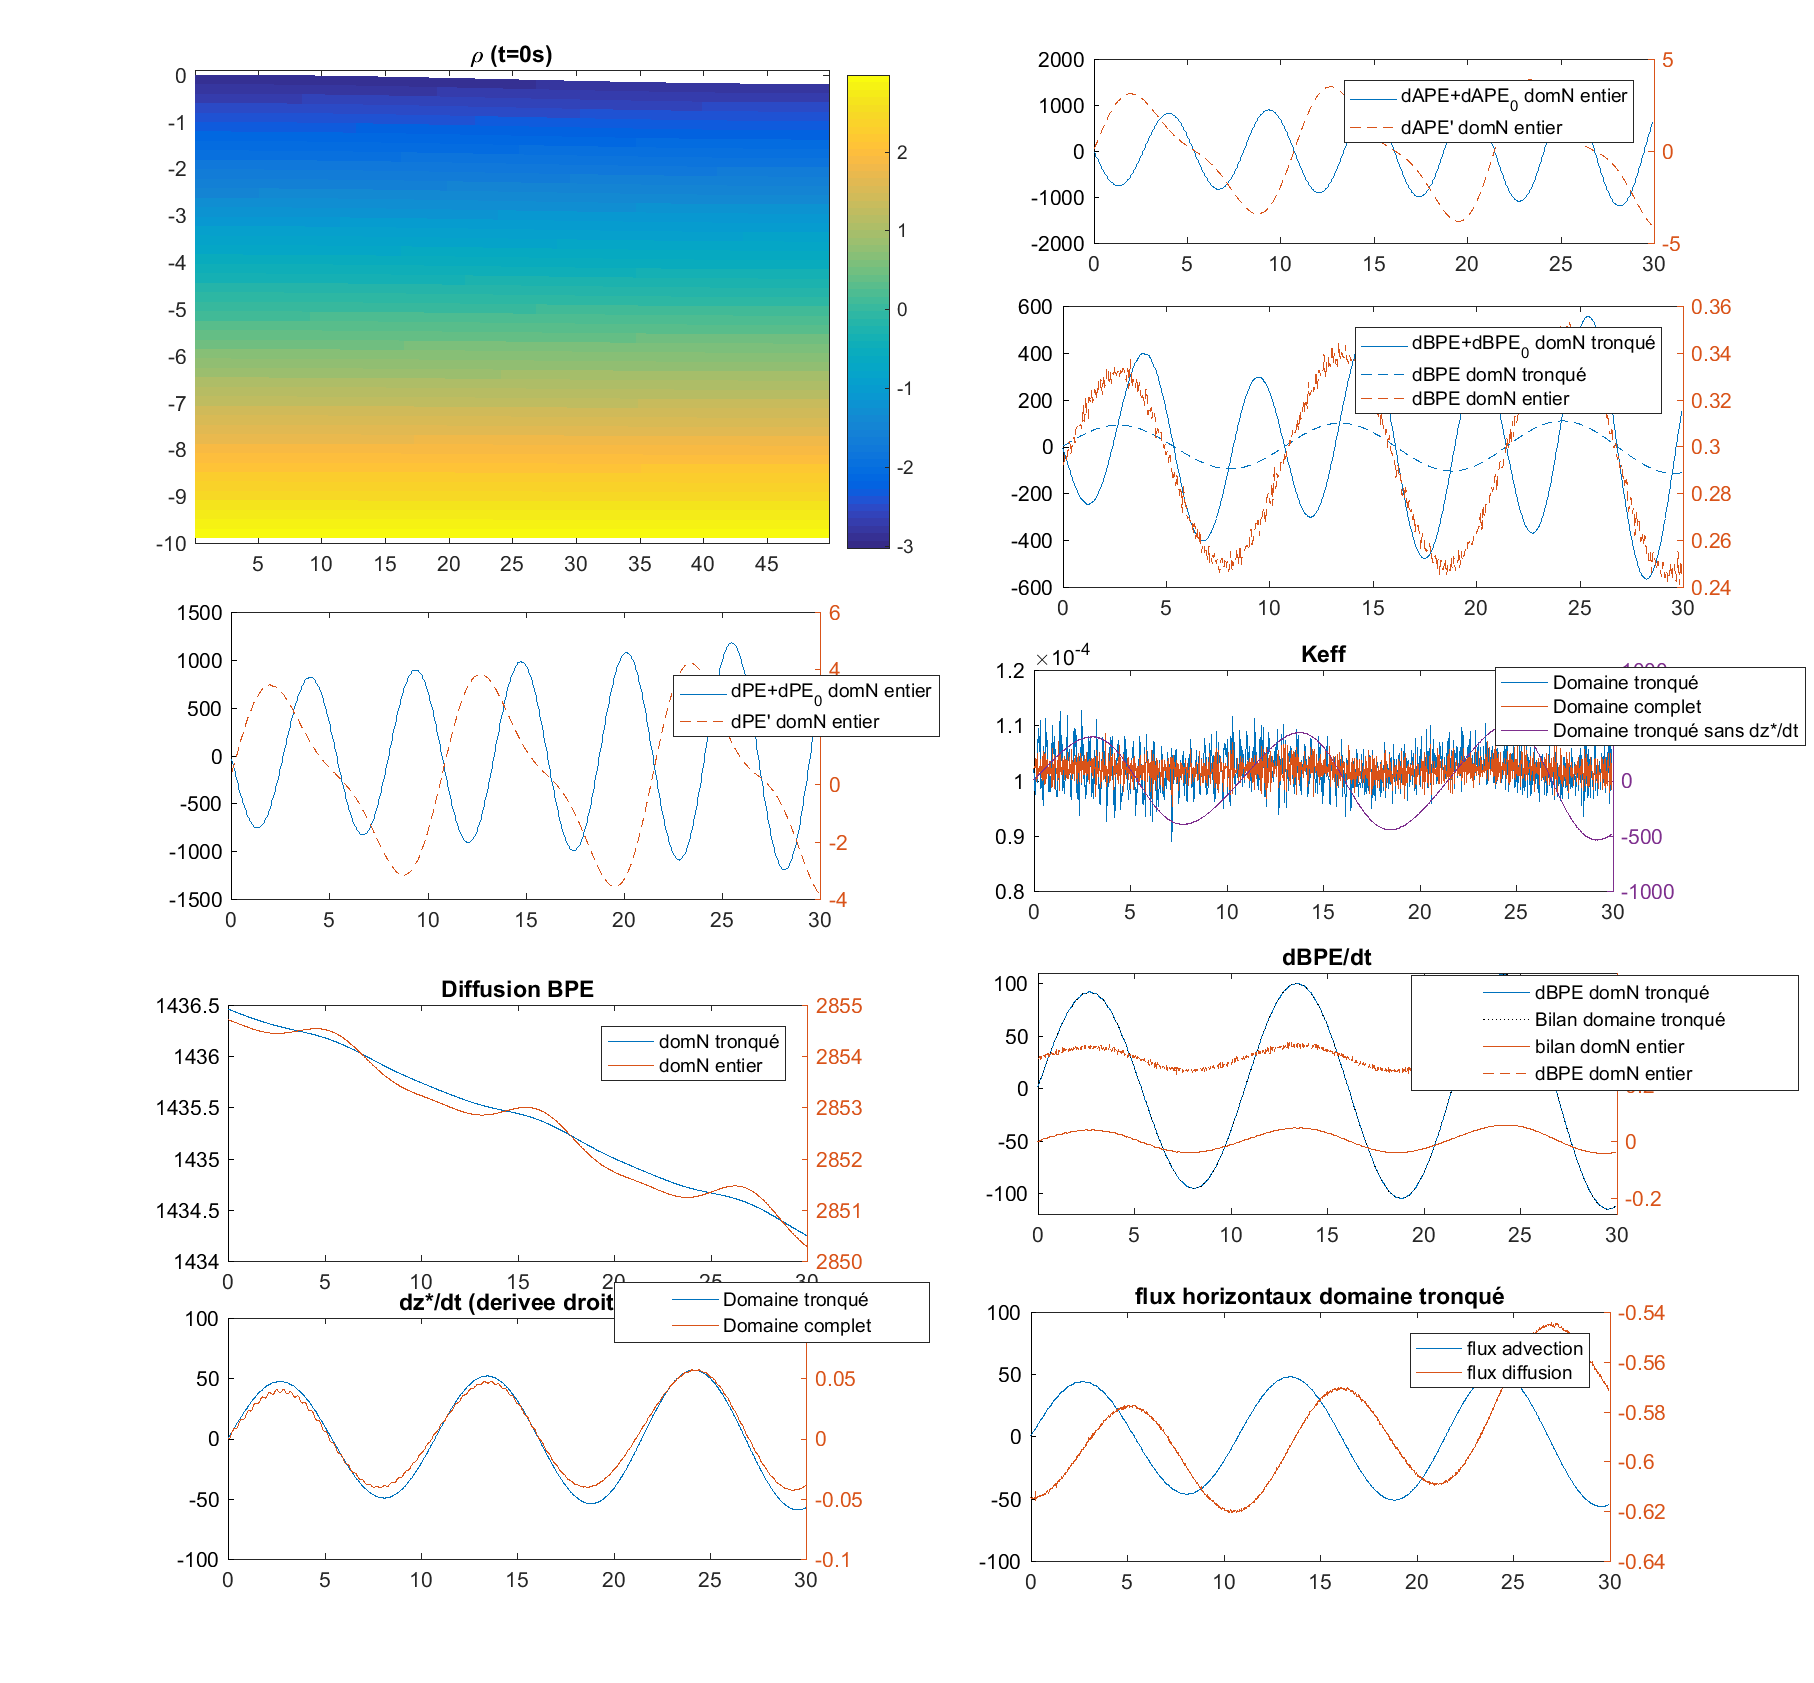
\includegraphics[width=1\textwidth]{./CHAP_BPE/AGBPE_numlab6.png}
\caption{Cas strat lineaire}
\label{figClin}
\end{figure}

\subsubsection{Pycnocline and free surface}

dx$=$dz$=$0.2m, L$=$50m, H$=$10m. Explicit coefficient put at $10^{-4}$m$^2$/s. Speed surface waves $\sqrt(gH)=5m/s$ and $T=5s$, interfacial wave $\sqrt(g'h_1h_2/H)=0.33m/s$ and $T=150s$
Initial stratification not in hydrostatic balance, waves travelling on the pycnocline.(Profile in vertical is tanh, add sinusoidal depandance in x). Initial disturbance of pycnocline depth several order greater than amplitude of free surface elevation, will have greater importance in energy balance.

Fig \ref{figCpsin}. Look at evaluation of $\kappa$ in whole domain, then in each half domain. In half domains, contribution of free surface($dz*/dt$) small compared to advection through the boundary.  When average value of $\kappa$ found for each half find the explicit value but locally oscillation around this value (high frequency : $2*T_{\text{surface}}$).

In each half domain, see increase in BPE (positive value of dBPE) when the depth of the interface increases, and respectively BPE will decrease as the interface gets shallower.

\begin{figure}[h!]
\centering
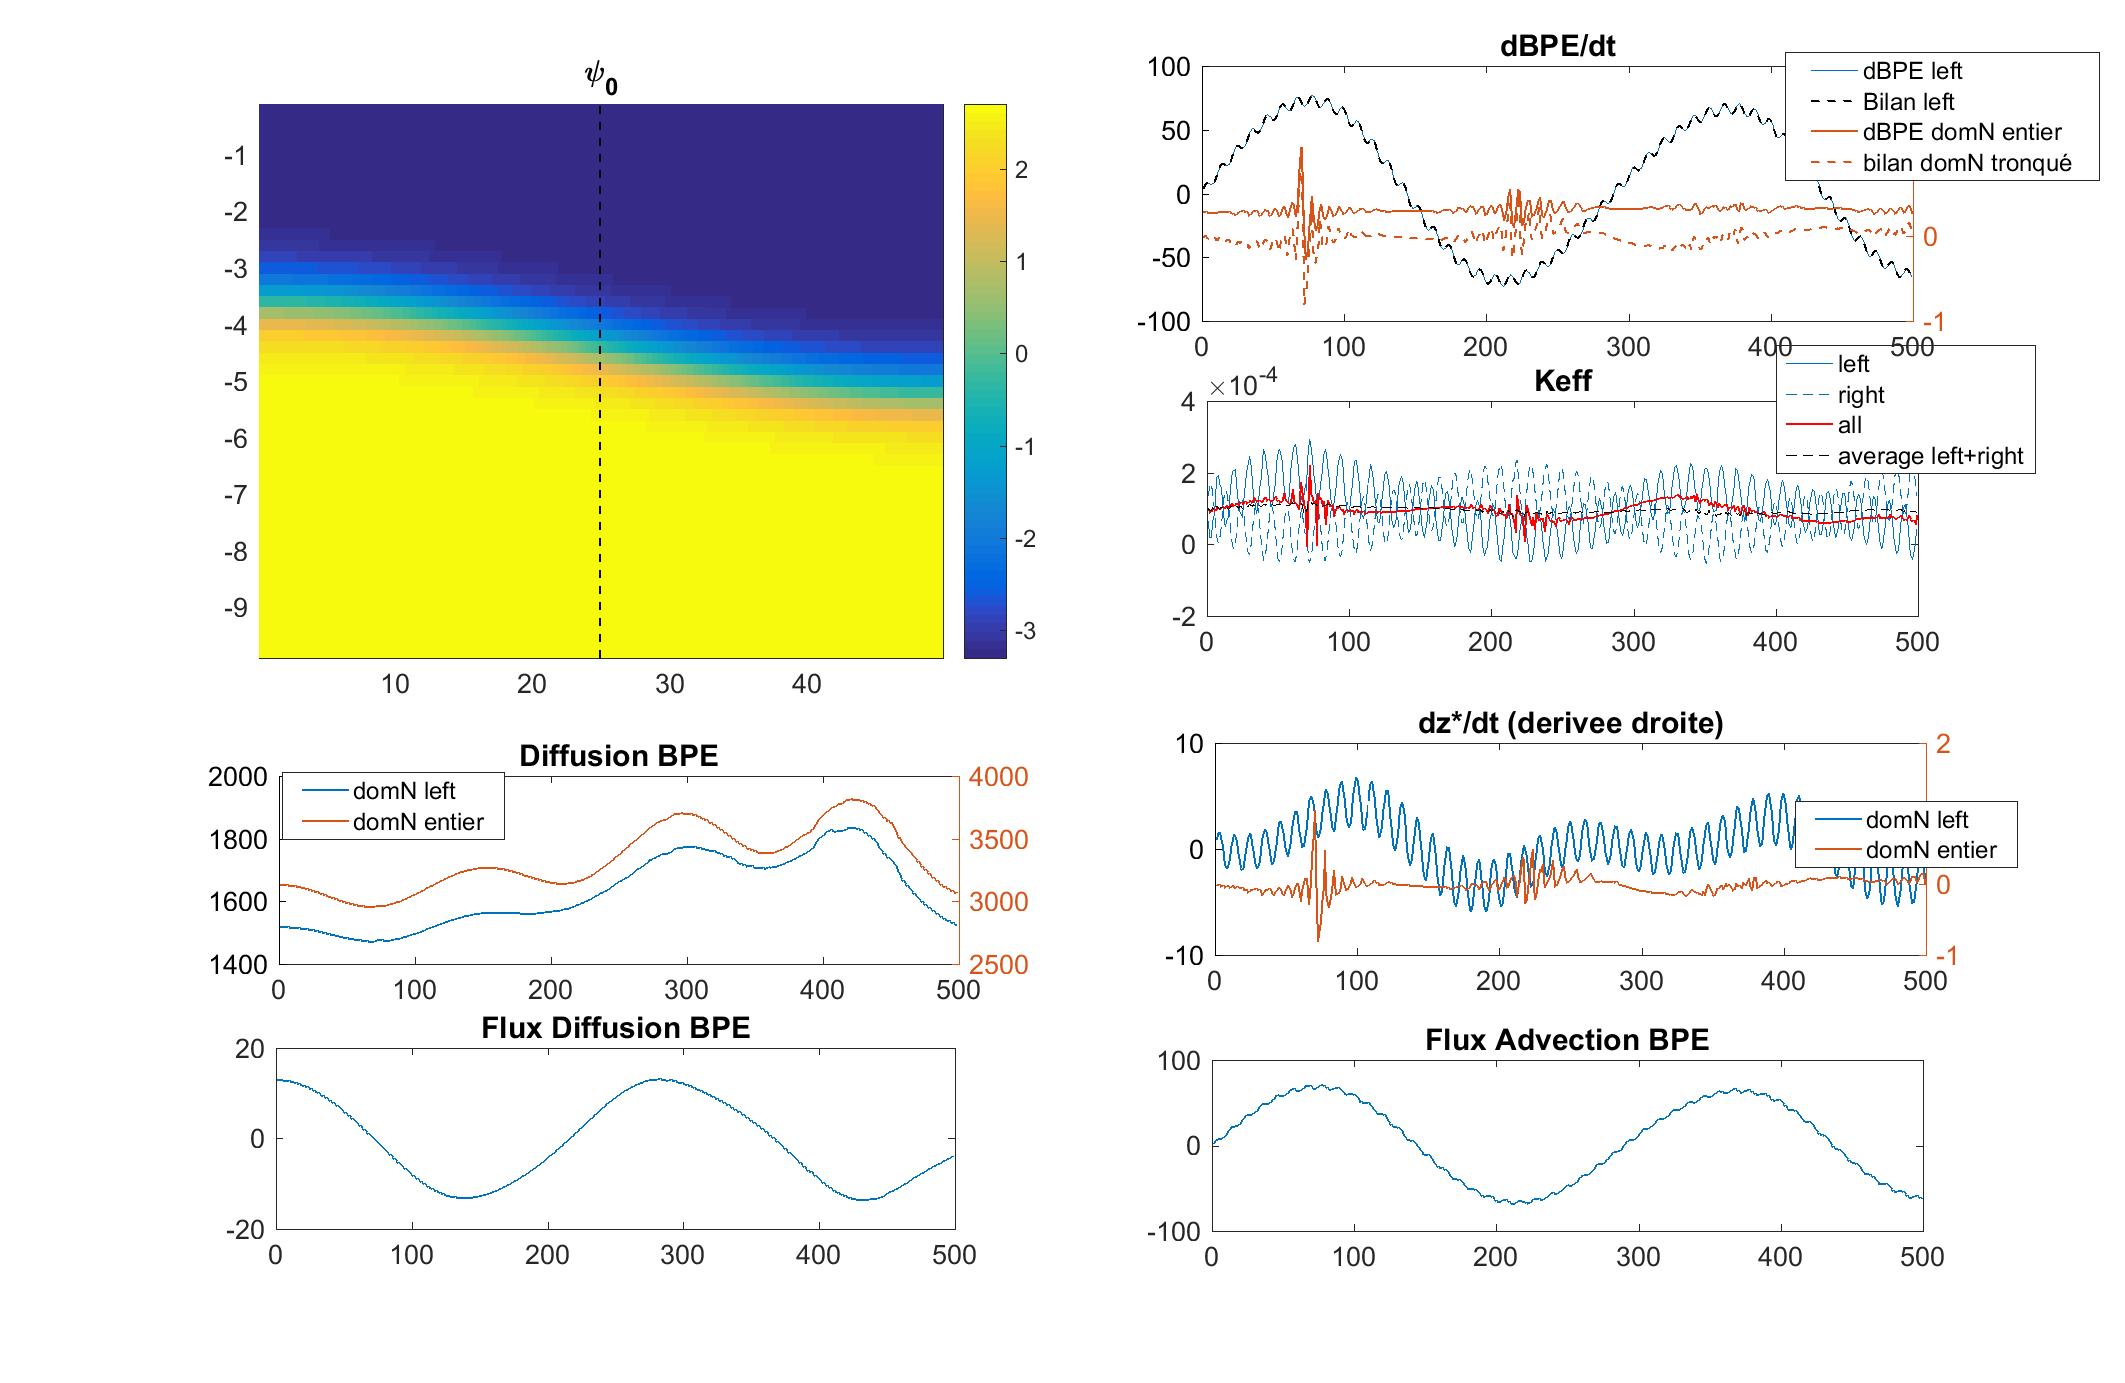
\includegraphics[width=1\textwidth]{./CHAP_BPE/AGBPE_numlab7.png}
\caption{TANK Pycnocline case.bottom row : advection and diffusion flux in regard to the left domain(as discussed in numlab part, do not cancel with fluxes computed for the right half)}
\label{figCpsin}
\end{figure}

In above figure output frequency is 1s.

Since compare instantaneous terms with temporal derivates in the balance of eq.(...), there is an impact of the time sampling on determination of $\kappa$. This is especially true if there is an open boundary, then the value of instantaneous advection through the boundary is the dominant term in the balance and close to $dBPE/dt$. If the sampling is to coarse, non-diffusive terms can be greater than $dBPE/dt$ and the balance will result in a negative value of $\kappa$.

\begin{figure}
\begin{subfigure}{.5\textwidth}
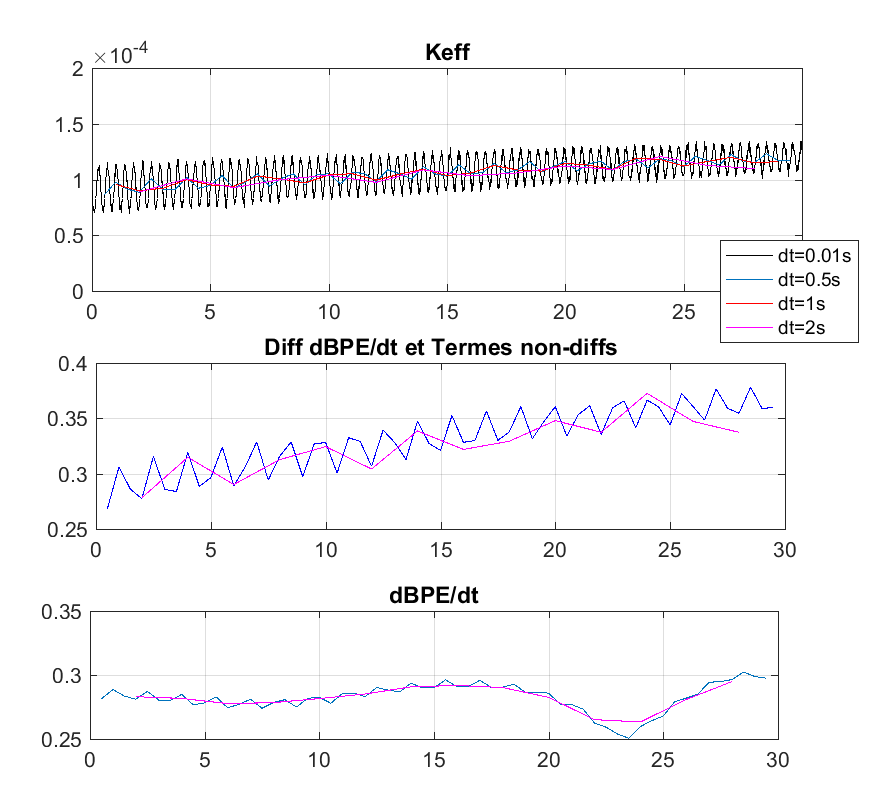
\includegraphics[width=1\textwidth]{./CHAP_BPE/figcompKAPPA_dt-out_psinAll.png}
\caption{In complete closed domain}
\end{subfigure}
\begin{subfigure}{.5\textwidth}
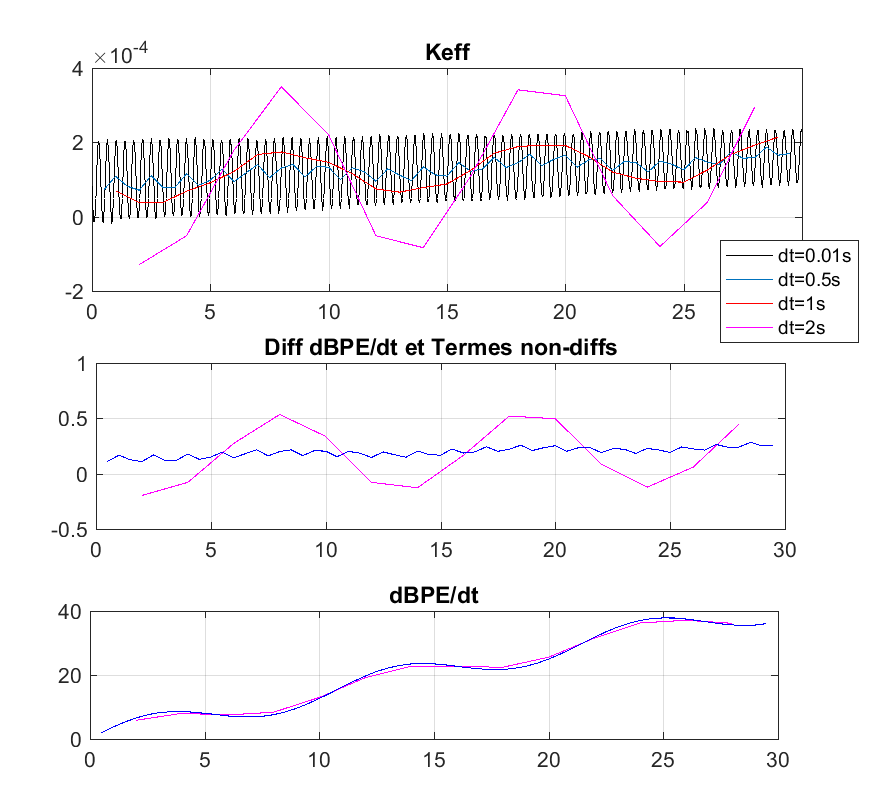
\includegraphics[width=1\textwidth]{./CHAP_BPE/figcompKAPPA_dt-out_psinL.png}
\caption{In left half domain (ie, with open boundary)}
\end{subfigure}
\caption{Pycno case, $\kappa$ for different time sampling/output frequency}
\end{figure}

\subsubsection{Pycnocline, free surface and bottom bathymetry}

Depth varies from 10m (dz$=$dx) at left boundary to 8.5m (dz$<$dx) at the right one. dx$=$0.2m. Explicit diffusion coefficient enabled $10^-4m^2/s$.

\begin{figure}[h!]

\begin{subfigure}{.5\textwidth}
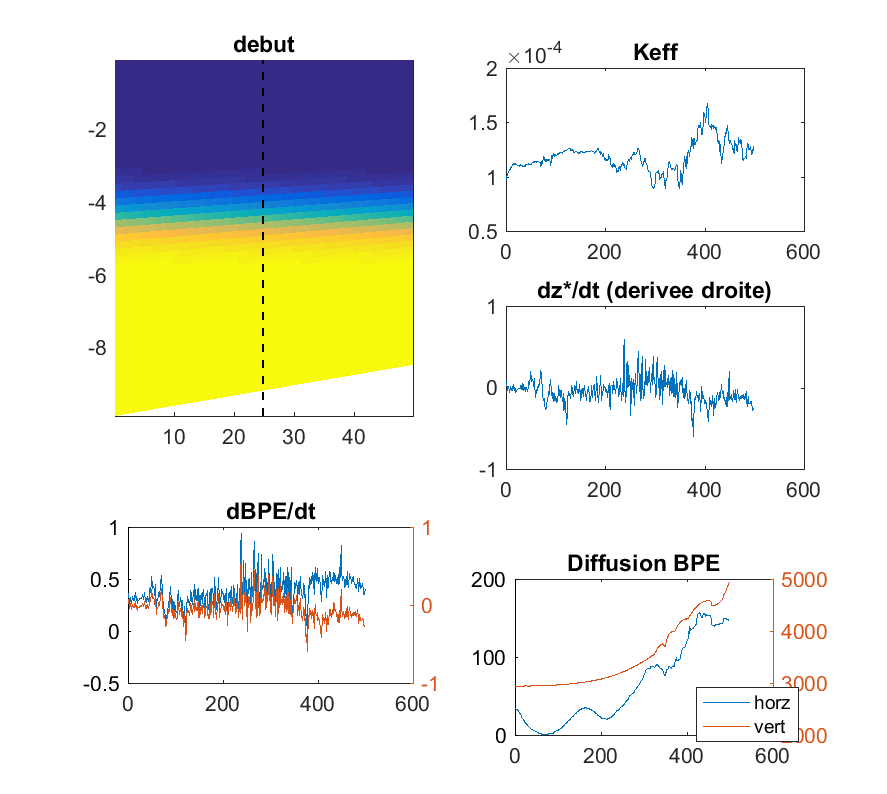
\includegraphics[width=1.\textwidth]{./CHAP_BPE/AGBPE_numlab9_all.png}
\caption{Closed domain}
%\label{figCkh}
\end{subfigure}
%
\begin{subfigure}{.5\textwidth}
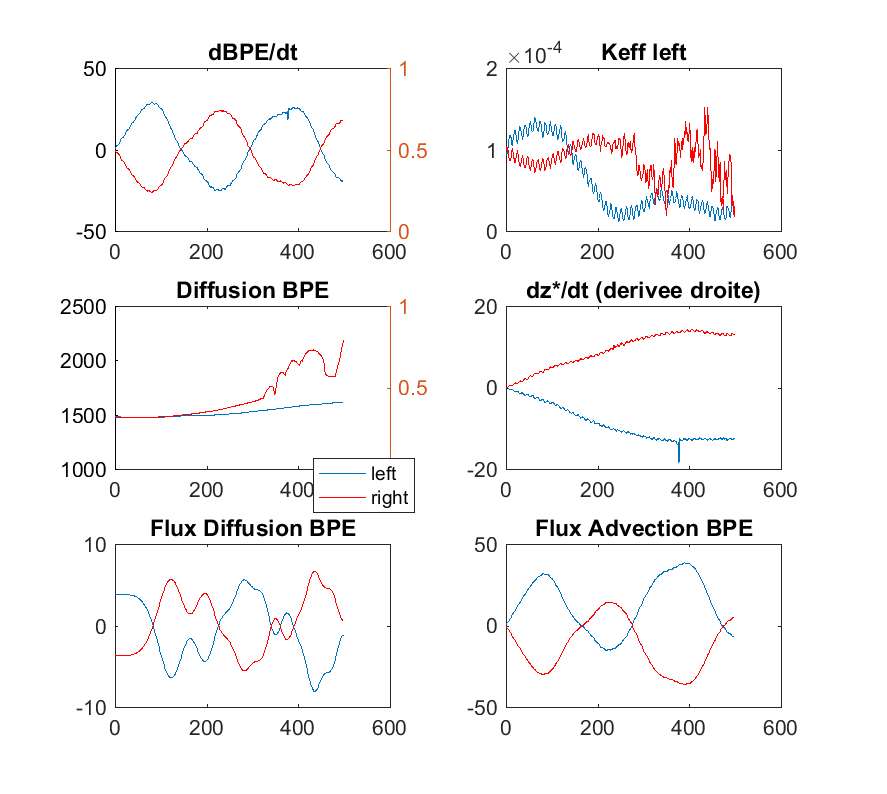
\includegraphics[width=1.\textwidth]{./CHAP_BPE/AGBPE_numlab9_halves.png}
\caption{half domains}
%\label{figCkh}
\end{subfigure}
\caption{Bottom bathy case}
\end{figure}

\subsubsection{Kelvin-Helmoltz Instability : local estimation and mixing event}

dx$=$dz$=$2m, amplitude cisaillement courant initial 2m/s, cyclic in x. Here $\kappa_{eff}$!$= \kappa_{exp}$, implicit diffusion $\kappa_{imp}$ from advection scheme as instability grows.

In this domain develop two billows. The dynamic of the areas of this two region is the same so whether make BPE diag on whole domain or half of it same results for coefficient( dBPE and the lefth-hand terms of balance are halved).
However can further make calculation on sub-division of a half domain as presented in fig \ref{figCkh}. Dynamic is different in domain a(red) and b(green), in particular the gradients of density and by extension the diffusive terms do not behave the same, with thinning of the pycnocline in area b between billows until t$=$500s, acting like local restratification process(that is not counterbalanced by other terms...). This leads to negative value of '$\kappa$' in area b while in area a stay close to evaluation in whole domain.

Can recreate estimate of coeff for the whole billow by averaging the two estimates pondered by the diffusive terms. 


\begin{figure}[h!]
\centering
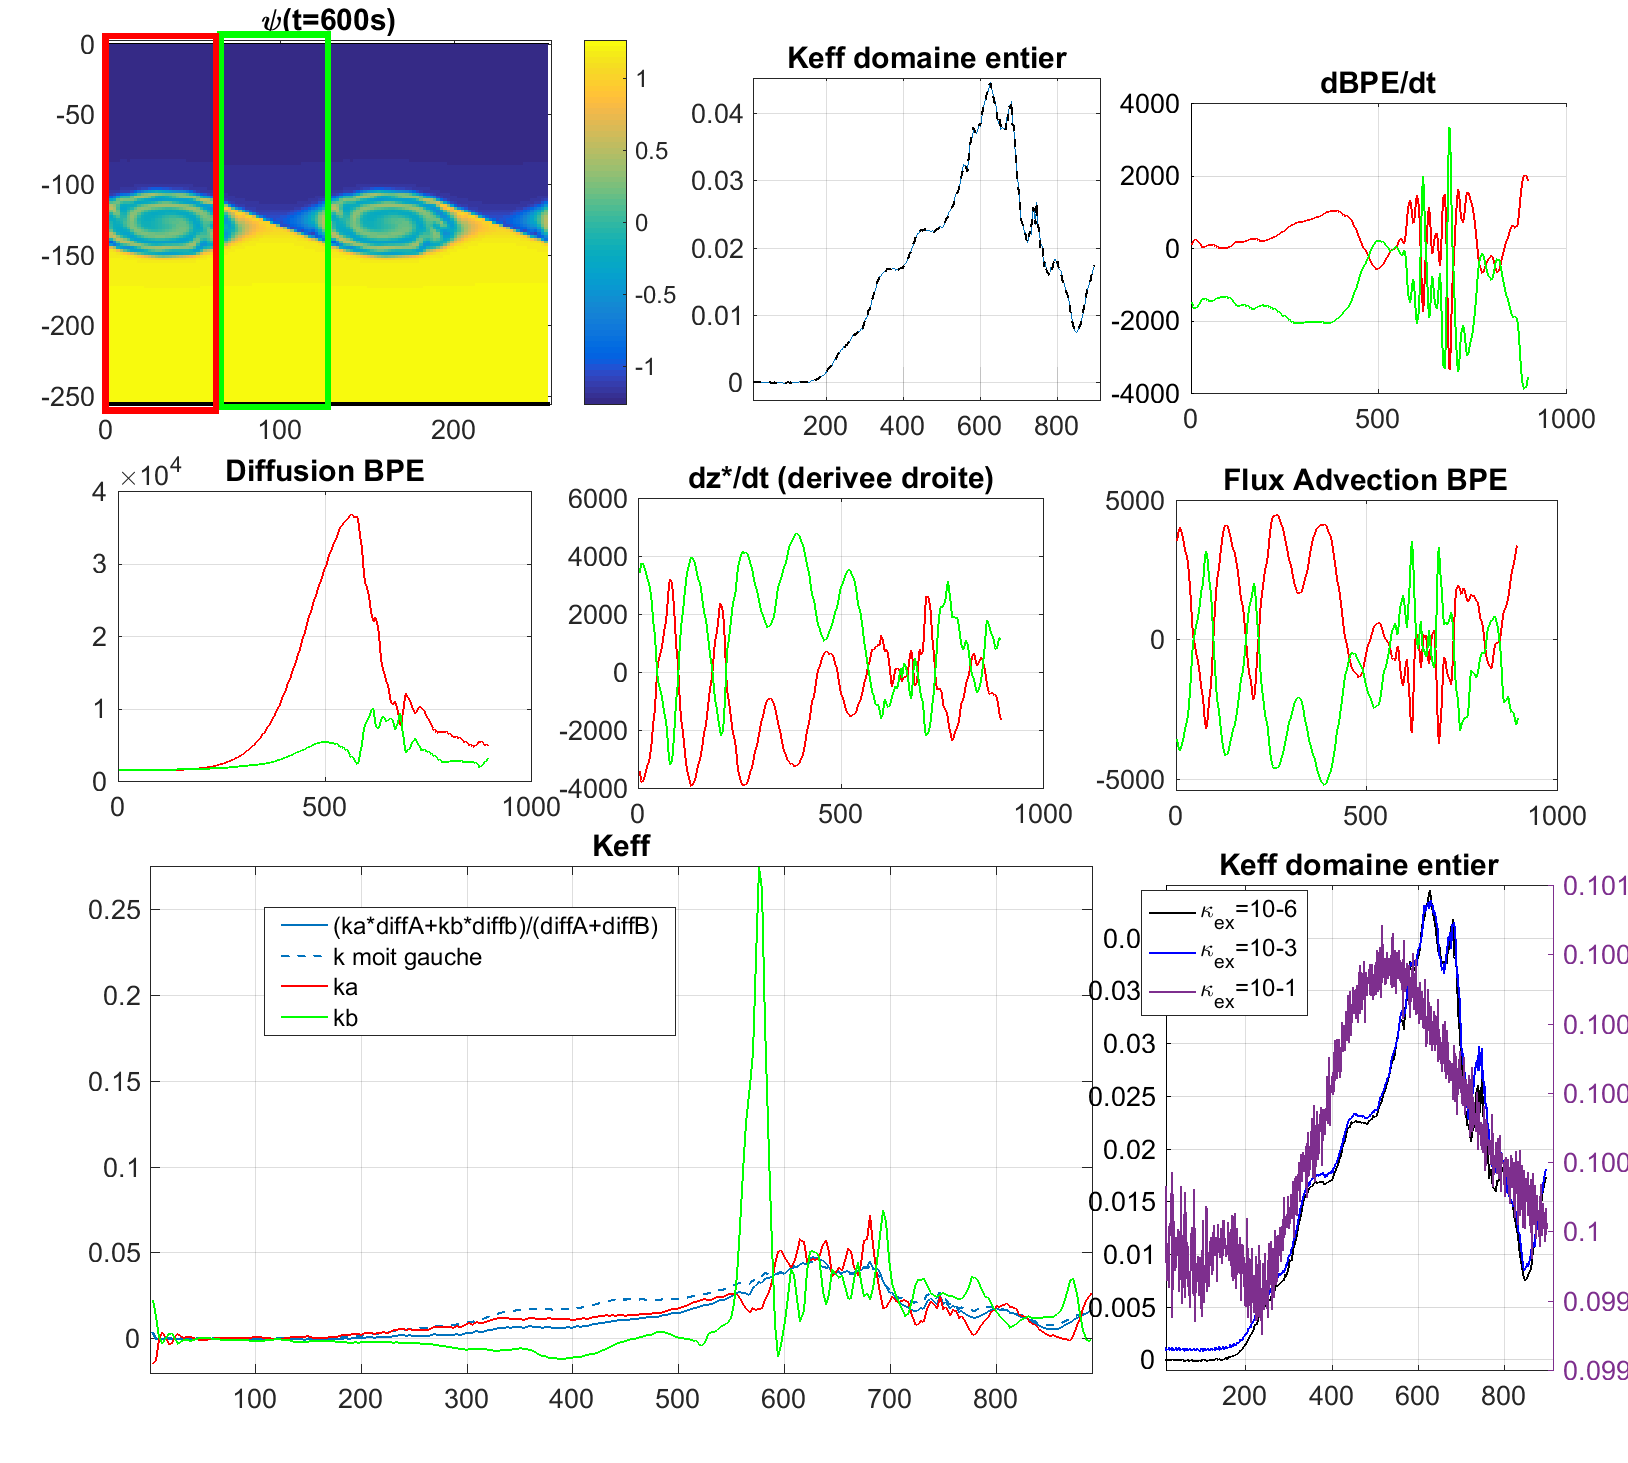
\includegraphics[width=1\textwidth]{./CHAP_BPE/AGBPE_numlab8-3c.png}
\caption{KH testcase. Domaine (a) rouge, (b) vert}
\label{figCkh}
\end{figure}


\newpage


%%%%%%%%%%%%%%%%%%%%%%%%%%%%%%%%%%%%%%%%%%%%%%%%%%%%%%%%%%%%%%%%%%%%%%%%%%%%%
%              Bibliography
%%%%%%%%%%%%%%%%%%%%%%%%%%%%%%%%%%%%%%%%%%%%%%%%%%%%%%%%%%%%%%%%%%%%%%%%%%%%%
%\bibliographystyle{apalike}
%%\bibliography{paper_agwaves}
%\bibliography{mybib}


